\documentclass[12pt,a4paper]{article}

\usepackage{fontspec}
\usepackage{polyglossia}
\setmainlanguage{vietnamese}
\setmainfont{Latin Modern Roman}
\usepackage[a4paper,left=2.8cm,right=2.2cm,top=2.5cm,bottom=2.5cm]{geometry}
\usepackage{setspace}
\onehalfspacing
\usepackage{graphicx}
\usepackage{booktabs}
\usepackage{tabularx}
\usepackage{array}
\usepackage{float}
\usepackage{xcolor}
\usepackage{hyperref}
\usepackage{tikz}
\usetikzlibrary{arrows.meta,positioning,shapes.geometric}
\usepackage{caption}
\usepackage{enumitem}
\usepackage{amsmath}
\usepackage{amssymb}

\hypersetup{
  colorlinks=true,
  linkcolor=blue!60!black,
  urlcolor=blue!60!black,
  citecolor=blue!60!black,
  pdftitle={Nghiên cứu và triển khai E-ELAN cho phân loại ảnh và phát hiện đối tượng},
  pdfauthor={Sinh viên thực hiện}
}

\newcommand{\projectname}{E-ELAN}
\newcommand{\classaccuracy}{91,12\%}

\begin{document}

\begin{titlepage}
\centering
{\large \textbf{TRƯỜNG ĐẠI HỌC KHOA HỌC TỰ NHIÊN}{\hspace{5cm}}}\\[0.3cm]
{\large \textbf{KHOA TOÁN CƠ TIN HỌC}{\hspace{5.5cm}}}\\[1.8cm]
{\Large \textbf{BÁO CÁO PROJECT}}\\[0.8cm]
{\LARGE \textbf{NGHIÊN CỨU VÀ TRIỂN KHAI KHỐI E-ELAN}}\\[0.35cm]
{\LARGE \textbf{CHO PHÂN LOẠI ẢNH VÀ PHÁT HIỆN ĐỐI TƯỢNG}}\\[1.5cm]

\begin{tikzpicture}[node distance=0.65cm, every node/.style={font=\small}]
\node[draw, rounded corners, fill=blue!8, minimum width=4.2cm, minimum height=0.8cm] (data) {Dataset cat/dog/panda};
\node[draw, rounded corners, fill=green!10, minimum width=4.2cm, minimum height=0.8cm, below=of data] (backbone) {E-ELAN Backbone};
\node[draw, rounded corners, fill=orange!12, minimum width=4.2cm, minimum height=0.8cm, below=of backbone] (neck) {FPN Neck};
\node[draw, rounded corners, fill=red!10, minimum width=4.2cm, minimum height=0.8cm, below=of neck] (head) {Detection Head};
\draw[-{Stealth}] (data)--(backbone);
\draw[-{Stealth}] (backbone)--(neck);
\draw[-{Stealth}] (neck)--(head);
\end{tikzpicture}\\[1.3cm]

\begin{center}
\begin{tabular}{@{}l l@{}}
\textbf{Sinh viên:} & NGUYỄN ANH ĐỨC \\[0.35cm]
\textbf{Mã sinh viên:} & 23001865 \\[0.35cm]
\textbf{Lớp học phần:} & MỘT SỐ VẤN ĐỀ CHỌN LỌC VỀ THỊ GIÁC MÁY TÍNH \\[0.35cm]
\textbf{Giảng viên:} & CAO VĂN CHUNG
\end{tabular}
\end{center}


\begin{center}
    {\large Tháng 10 năm 2026}
\end{center}
\end{titlepage}
\pagenumbering{roman}
\tableofcontents
\newpage
\pagenumbering{arabic}

\section{Đặt vấn đề}

Trong các hệ thống thị giác máy tính hiện đại, mạng nơ-ron tích chập đóng vai trò quan trọng trong việc trích xuất đặc trưng từ ảnh. Với bài toán phân loại ảnh, mô hình cần ánh xạ toàn bộ ảnh vào một nhãn lớp. Với bài toán phát hiện đối tượng, mô hình đồng thời phải xác định lớp và vị trí của từng đối tượng thông qua bounding box. Hai bài toán có yêu cầu đầu ra khác nhau nhưng có thể dùng chung một mạng trích xuất đặc trưng.

E-ELAN (Extended Efficient Layer Aggregation Network) là một ý tưởng kiến trúc được sử dụng trong họ mô hình YOLOv7. E-ELAN kế thừa tư tưởng mở rộng, kết hợp và trộn đặc trưng của ELAN, nhằm tăng khả năng học đặc trưng mà vẫn kiểm soát chi phí tính toán. Trong phạm vi mini project, mục tiêu không phải sao chép toàn bộ YOLOv7 mà là xây dựng một phiên bản có cấu trúc rõ ràng để khảo sát vai trò của E-ELAN.

Project được triển khai theo hai phần. Phần thứ nhất xây dựng mô hình phân loại ba lớp \textit{cat}, \textit{dog} và \textit{panda}, đồng thời thực hiện lưu trọng số, inference và đánh giá bằng các độ đo phân loại. Phần thứ hai sử dụng E-ELAN làm Backbone, kết hợp FPN Neck và Detection Head một-scale để tạo detector YOLO-style tối giản. Detector được huấn luyện trên dữ liệu có bounding box và đánh giá bằng precision, recall, F1-score và mAP@50.

\subsection{Mục tiêu}
\begin{itemize}[leftmargin=*]
  \item Phân tích cấu trúc và nguyên lý hoạt động của khối E-ELAN.
  \item Xây dựng mô hình phân loại ảnh ba lớp dựa trên E-ELAN.
  \item Xây dựng detector gồm Backbone, Neck và Head.
  \item Chuẩn hóa dữ liệu, tổ chức quy trình train, lưu weights và inference.
  \item Đánh giá kết quả, phân tích hiện tượng overfitting và các giới hạn của kiến trúc.
\end{itemize}

\section{Cơ sở lý thuyết}

\subsection{Mạng tích chập}

Mạng tích chập gồm các lớp convolution, normalization và hàm kích hoạt. Lớp convolution học các bộ lọc để phát hiện cạnh, góc, họa tiết và các cấu trúc có mức độ phức tạp tăng dần. Batch Normalization giúp ổn định phân phối kích hoạt, trong khi SiLU cung cấp hàm kích hoạt trơn, thường phù hợp với các mô hình thị giác hiện đại.

\subsection{Tư tưởng ELAN và E-ELAN}

ELAN tổ chức nhiều nhánh xử lý với độ sâu khác nhau, sau đó ghép các đặc trưng để tăng đa dạng đường truyền gradient. E-ELAN mở rộng ý tưởng này bằng cách duy trì khả năng học của các nhóm đặc trưng, kết hợp các nhánh song song và thực hiện channel shuffle để trao đổi thông tin giữa các nhóm.

Một block E-ELAN rút gọn trong project gồm các thành phần:
\begin{enumerate}[leftmargin=*]
  \item Nhánh mở rộng kênh bằng convolution $1\times1$ có group.
  \item Tách tensor thành các nhóm kênh.
  \item Các nhánh song song gồm identity, một convolution $3\times3$ và chuỗi convolution sâu hơn.
  \item Ghép các nhánh theo chiều kênh.
  \item Trộn kênh và chiếu về số kênh ban đầu.
  \item Kết nối residual giữa đầu vào và đầu ra.
\end{enumerate}

Nếu đầu vào của block là $X$, phép biến đổi có thể mô tả khái quát:
\[
Y = X + \mathcal{P}\left(\operatorname{Concat}
    \left(B_1(G(X)),B_2(G(X)),B_3(G(X))\right)\right),
\]
trong đó $G$ là phép mở rộng theo nhóm, $B_i$ là các nhánh xử lý, còn $\mathcal{P}$ là phép chiếu sau khi ghép.

\subsection{Backbone, Neck và Detection Head}

Backbone chịu trách nhiệm trích xuất đặc trưng. Neck kết hợp các đặc trưng ở những mức phân giải khác nhau, giúp detector sử dụng được cả thông tin ngữ nghĩa cấp cao và thông tin không gian. Detection Head chuyển đặc trưng thành dự đoán bounding box, objectness và xác suất lớp.

Trong project, Backbone tạo ra ba mức đặc trưng tương ứng với các tầng $P3$, $P4$ và $P5$. FPN Neck chiếu đặc trưng $P5$ về số kênh phù hợp, nội suy lên kích thước của $P4$ và cộng với $P4$. Head một-scale dự đoán trên bản đồ lưới $32\times32$. Mỗi ô lưới chứa bốn giá trị hộp, một objectness và ba điểm lớp.

\section{Phương pháp và kiến trúc đề xuất}

\subsection{Quy trình tổng thể}

Quy trình thực nghiệm gồm các bước:
\begin{enumerate}[leftmargin=*]
  \item Chuẩn hóa dữ liệu phân loại và phát hiện.
  \item Kiểm tra ảnh, nhãn, bounding box và phân chia train/validation/test.
  \item Xây dựng các module convolution, E-ELAN, Backbone, Neck và Head.
  \item Kiểm tra forward pass và loss trên một batch.
  \item Overfit trên một tập con nhỏ để xác nhận pipeline học được.
  \item Train đầy đủ, lưu checkpoint có validation loss thấp nhất.
  \item Decode dự đoán, lọc confidence, NMS và đánh giá trên test set.
\end{enumerate}

\subsection{Dữ liệu}

Nhãn được thống nhất thành:
\[
0=\text{cat},\qquad 1=\text{dog},\qquad 2=\text{panda}.
\]

Đối với classification, dữ liệu được tổ chức theo cấu trúc thư mục của ImageFolder. Đối với detection, dữ liệu sử dụng định dạng YOLO, trong đó mỗi dòng có dạng $(c,x_c,y_c,w,h)$ và các tọa độ được chuẩn hóa về đoạn $[0,1]$.

\begin{table}[H]
\centering
\caption{Thống kê dataset detection}
\begin{tabular}{lrrr}
\toprule
\textbf{Split} & \textbf{Ảnh} & \textbf{Nhãn} & \textbf{Bounding box}\\
\midrule
Train & 3108 & 3108 & 3921\\
Validation & 583 & 583 & 703\\
Test & 500 & 500 & 629\\
\midrule
Tổng & 4191 & 4191 & 5253\\
\bottomrule
\end{tabular}
\end{table}

\subsection{Kiến trúc Backbone}

Ảnh đầu vào có kích thước $256\times256$. Stem giảm kích thước không gian và tăng số kênh. Các stage tiếp theo lần lượt giảm độ phân giải, tăng số kênh và áp dụng E-ELAN block. Cấu trúc khái quát:

\begin{table}[H]
\centering
\caption{Các mức đặc trưng của Backbone}
\begin{tabular}{lccc}
\toprule
\textbf{Mức} & \textbf{Độ phân giải tương đối} & \textbf{Số kênh} & \textbf{Vai trò}\\
\midrule
Stem & $1/2$ & 32 & Đặc trưng ban đầu\\
$P3$ & $1/4$ & 64 & Chi tiết không gian\\
$P4$ & $1/8$ & 128 & Đặc trưng trung gian\\
$P5$ & $1/16$ & 256 & Ngữ nghĩa cấp cao\\
\bottomrule
\end{tabular}
\end{table}

\subsection{FPN Neck}

FPN Neck dùng phép chiếu $1\times1$ cho $P5$ và $P4$, nội suy $P5$ lên cùng kích thước với $P4$, sau đó cộng hai tensor. Một convolution $3\times3$ được dùng để trộn đặc trưng sau khi hợp nhất. Cách thiết kế này đơn giản nhưng minh họa được vai trò của Neck trong việc truyền thông tin từ tầng sâu về tầng có độ phân giải cao hơn.

\subsection{Detection Head và hàm mất mát}

Detection Head tạo tensor có kích thước:
\[
B\times(5+C)\times S\times S
= B\times8\times32\times32,
\]
với $C=3$ lớp. Bốn kênh đầu mô tả vị trí và kích thước hộp, kênh thứ năm là objectness, ba kênh còn lại là điểm lớp.

Target được mã hóa vào ô lưới chứa tâm bounding box. Hàm mất mát gồm ba nhóm chính: Smooth L1 cho hộp, binary cross entropy cho objectness và binary cross entropy cho class score. Objectness ở các ô không có đối tượng được phạt để giảm dự đoán nền.

\subsection{Inference và đánh giá}

Trong inference, đầu ra raw được chuyển thành tâm và kích thước bounding box, sau đó đưa về hệ tọa độ chuẩn hóa. Confidence được tính bằng tích giữa objectness và điểm lớp lớn nhất. Các dự đoán dưới ngưỡng confidence bị loại. Non-Maximum Suppression được áp dụng riêng theo từng lớp để loại các hộp chồng lấn.

Với một dự đoán và một ground truth, IoU được tính:
\[
\operatorname{IoU}=\frac{\operatorname{Area}(B_p\cap B_g)}
{\operatorname{Area}(B_p\cup B_g)}.
\]
Một dự đoán được xem là đúng khi cùng lớp và IoU không nhỏ hơn $0.5$.

\section{Thực nghiệm}

\subsection{Thiết lập}

Thực nghiệm được chạy trên Windows với Python 3.13.14, PyTorch 2.12.0, torchvision 0.27.0, ảnh resize về $256\times256$, optimizer AdamW và batch size 16. Classification sử dụng dataset crop theo ba thư mục lớp. Detection sử dụng dataset YOLO đã chuẩn hóa.

\subsection{Kết quả classification}

Mô hình classification đạt accuracy trên test khoảng \classaccuracy. Kết quả theo lớp:

\begin{table}[H]
\centering
\caption{Kết quả classification trên tập test}
\begin{tabular}{lrrr}
\toprule
\textbf{Lớp} & \textbf{Precision} & \textbf{Recall} & \textbf{F1-score}\\
\midrule
Cat & 77,78\% & 96,55\% & 86,15\%\\
Dog & 97,18\% & 89,15\% & 92,99\%\\
Panda & 89,17\% & 92,24\% & 90,68\%\\
\bottomrule
\end{tabular}
\end{table}

Kết quả cho thấy mô hình nhận diện dog tốt nhất về precision. Cat có recall cao, nghĩa là phần lớn ảnh cat được phát hiện đúng nhưng vẫn có một số ảnh lớp khác bị dự đoán nhầm thành cat. Panda đạt kết quả cân bằng hơn giữa precision và recall.

\begin{figure}[H]
\centering
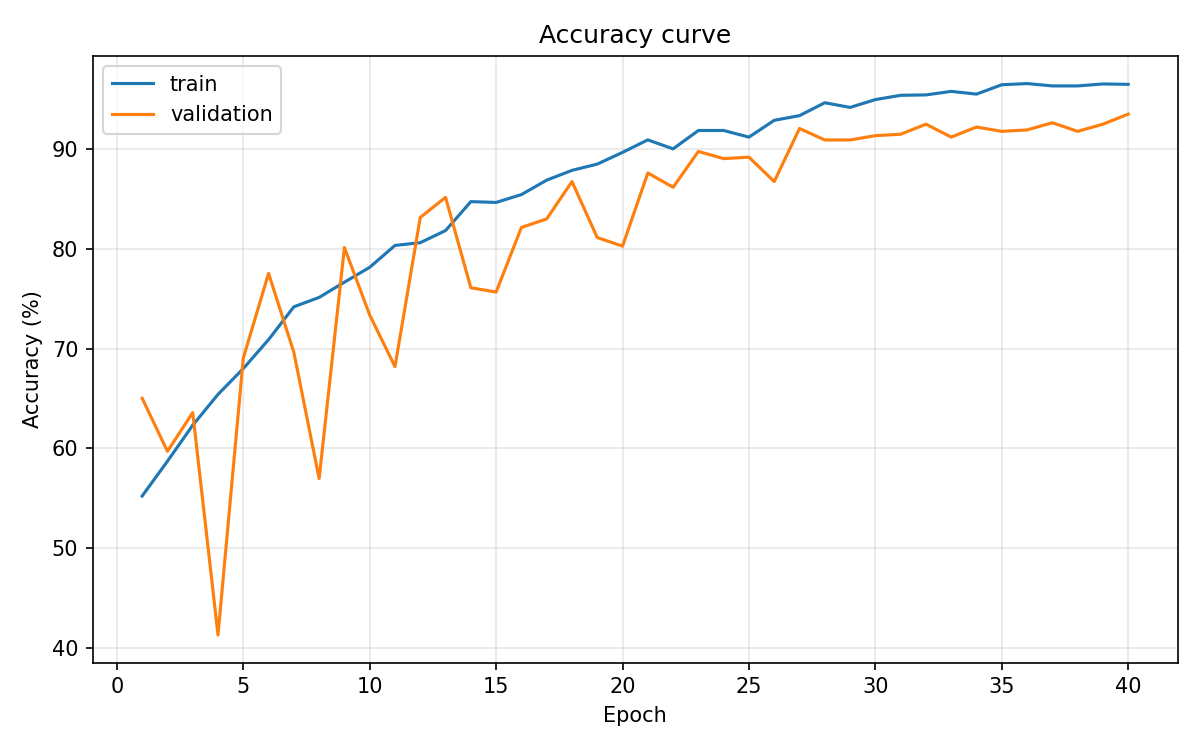
\includegraphics[width=0.78\textwidth]{classification/outputs/cls_eelan_improved/plots/accuracy_curve.png}
\caption{Đường cong accuracy trong quá trình huấn luyện classification}
\end{figure}

\begin{figure}[H]
\centering
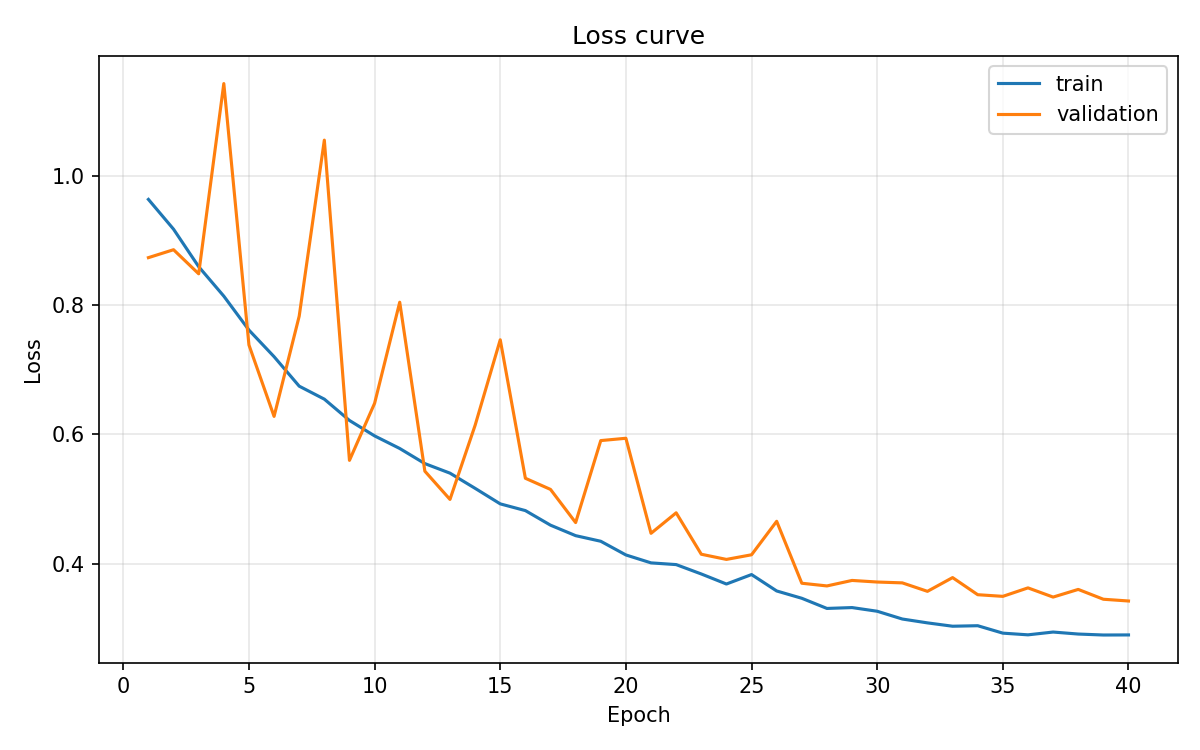
\includegraphics[width=0.78\textwidth]{classification/outputs/cls_eelan_improved/plots/loss_curve.png}
\caption{Đường cong loss trong quá trình huấn luyện classification}
\end{figure}

\subsection{Kiểm tra overfit detection}

Trên 10 ảnh, loss giảm từ $1,7981$ xuống $0,0091$. Đây là kiểm tra quan trọng để xác nhận target encoding, forward pass, gradient và optimizer hoạt động. Kết quả không đại diện cho khả năng tổng quát hóa nhưng chứng minh pipeline có thể học dữ liệu.

\subsection{Kết quả detection}

Detection được train 15 epoch với learning rate $3\times10^{-4}$ và weight decay $10^{-4}$. Validation loss tốt nhất ở epoch 2:

\begin{table}[H]
\centering
\caption{Một số mốc validation loss}
\begin{tabular}{lrr}
\toprule
\textbf{Epoch} & \textbf{Train loss} & \textbf{Validation loss}\\
\midrule
1 & 0,9952 & 1,0135\\
2 & 0,6872 & 0,8600\\
5 & 0,3129 & 0,9791\\
10 & 0,1338 & 1,8745\\
15 & 0,0976 & 2,3942\\
\bottomrule
\end{tabular}
\end{table}

Checkpoint tốt nhất được lựa chọn theo validation loss thay vì sử dụng checkpoint cuối. Cách chọn này hạn chế ảnh hưởng của overfitting.

Đánh giá cuối dùng confidence threshold $0,75$, IoU threshold $0,50$ và tối đa 20 detection trên mỗi ảnh:

\begin{table}[H]
\centering
\caption{Kết quả detection trên tập test}
\begin{tabular}{lr}
\toprule
\textbf{Độ đo} & \textbf{Giá trị}\\
\midrule
Precision & 4,83\%\\
Recall & 22,58\%\\
F1-score & 7,95\%\\
mAP@50 & 11,63\%\\
\midrule
True Positive & 142\\
False Positive & 2800\\
False Negative & 487\\
\bottomrule
\end{tabular}
\end{table}

\begin{table}[H]
\centering
\caption{AP@50 theo lớp}
\begin{tabular}{lr}
\toprule
\textbf{Lớp} & \textbf{AP@50}\\
\midrule
Cat & 0,2178\\
Dog & 0,0909\\
Panda & 0,0402\\
\bottomrule
\end{tabular}
\end{table}

\section{Đánh giá và nhận xét}

\subsection{Ưu điểm}
\begin{itemize}[leftmargin=*]
  \item Pipeline được xây dựng xuyên suốt từ dữ liệu đến inference.
  \item E-ELAN được tách thành block riêng, dễ phân tích và tái sử dụng.
  \item Có sự phân tách rõ giữa Backbone, Neck và Head.
  \item Có checkpoint tốt nhất, biểu đồ loss và các độ đo định lượng.
  \item Classification cho kết quả tốt, accuracy vượt 90\%.
  \item Quy trình overfit giúp phát hiện sớm lỗi trong target hoặc loss.
\end{itemize}

\subsection{Hạn chế}

Kết quả detection thấp hơn classification đáng kể. Precision chỉ đạt $4,83\%$ và mAP@50 đạt $11,63\%$. Nguyên nhân chính là detector đang ở mức tối giản: chỉ dự đoán một-scale, mỗi ô lưới chỉ mã hóa một object, Head không có đầy đủ cơ chế anchor hoặc multi-scale như các detector hiện đại, và hàm mất mát chưa bao gồm các thành phần IoU nâng cao như GIoU hoặc CIoU.

Validation loss tăng sau epoch 2 trong khi train loss tiếp tục giảm, cho thấy overfitting. Dữ liệu panda cũng có AP thấp nhất, gợi ý cần kiểm tra thêm độ đa dạng, chất lượng annotation và cân bằng dữ liệu của lớp này.

Metric mAP@50 trong notebook là metric tự cài đặt nhằm minh họa quy trình. Nó không nên được diễn giải là COCO mAP chuẩn. Khi so sánh nghiêm túc, cần dùng một thư viện đánh giá chuẩn và định dạng kết quả tương ứng.

\subsection{Hướng cải thiện}
\begin{enumerate}[leftmargin=*]
  \item Sử dụng multi-scale detection head để xử lý đối tượng lớn nhỏ khác nhau.
  \item Cho phép nhiều prediction trên một ô lưới hoặc chuyển sang thiết kế anchor-free đầy đủ.
  \item Bổ sung GIoU/CIoU loss, focal loss và cơ chế cân bằng objectness.
  \item Tăng cường dữ liệu bằng lật ảnh, biến đổi màu và biến đổi hình học có kiểm soát.
  \item Dùng learning-rate scheduler và early stopping dựa trên validation metric.
  \item Chuẩn hóa đánh giá bằng COCO API hoặc TorchMetrics.
  \item Kiểm tra riêng annotation và chất lượng ảnh của lớp panda.
\end{enumerate}

\section{Kết luận}

Project đã xây dựng được một quy trình hoàn chỉnh để nghiên cứu E-ELAN cho hai bài toán phân loại ảnh và phát hiện đối tượng. Ở phần classification, E-ELAN cho kết quả tốt với accuracy test khoảng \classaccuracy. Ở phần detection, E-ELAN được sử dụng làm Backbone và kết hợp với FPN Neck cùng Detection Head một-scale. Pipeline đã thực hiện được train, lưu checkpoint, decode, NMS và đánh giá.

Kết quả detection còn thấp nhưng phù hợp với mục tiêu minh họa một detector tự xây dựng và giúp chỉ ra rõ tác động của thiết kế Backbone--Neck--Head, target encoding và lựa chọn ngưỡng inference. Các hạn chế đã được xác định cụ thể, tạo cơ sở cho các hướng phát triển tiếp theo.

\section{Tài liệu tham khảo}
\begin{enumerate}[leftmargin=*]
  \item C.-Y. Wang và cộng sự, ``YOLOv7: Trainable bag-of-freebies sets new state-of-the-art for real-time object detectors,'' arXiv:2207.02696, 2022.
  \item T.-Y. Lin và cộng sự, ``Feature Pyramid Networks for Object Detection,'' Proceedings of CVPR, 2017.
  \item K. He và cộng sự, ``Deep Residual Learning for Image Recognition,'' Proceedings of CVPR, 2016.
  \item J. Redmon và cộng sự, ``You Only Look Once: Unified, Real-Time Object Detection,'' Proceedings of CVPR, 2016.
  \item A. Paszke và cộng sự, ``PyTorch: An Imperative Style, High-Performance Deep Learning Library,'' Advances in Neural Information Processing Systems, 2019.
  \item Tài liệu môn học và file \textit{Advanced\_CV.pdf} được cung cấp trong project.
  \item Tài liệu chính thức của torchvision về transforms, dataset và object detection operators.
\end{enumerate}

\end{document}
